\documentclass[12pt]{gost-7-32}

\usepackage{indentfirst}
\usepackage{amssymb}
\usepackage{amsmath}
\usepackage{graphicx}
\usepackage{color}
\usepackage{array}
\usepackage{tabularx}

\usepackage{listings}
\lstset{
    basicstyle=\ttfamily
}

\begin{document}

\sloppy

\essay

Пояснительная записка содержит: 35 страницы, 1 рисунок, 19 ссылок на источники и 2 приложения.

РАСПОЗНАВАНИЕ ГОЛОСА, МОШЕННИЧЕСТВО, МАШИННОЕ  ОБУЧЕНИЕ, МОДЕЛЬ ГАУССОВЫХ СМЕСЕЙ, МАКСИМИЗАЦИЯ ОЖИДАНИЯ.

Объектом исследования являются техники голосовой идентификации и их точность.

Цель работы: реализация прототипа программного продукта голосовой аутентификации на основе модели гауссовых смесей.

Результаты работы: изучены основные методы голосовой идентификации.
Определены ключевые характеристики метода, требуемые для голосовой идентификации мошенника в условиях телефонного разговора.
Реализованы базовые прототипы программных продуктов распознавания пола и личности человека по голосу.

Полученные результаты обеспечивают стойкую математическую основу для построения более сложных схем распознавания голоса.
Реализованные программные продукты могут с незначительными изменениями быть использованы в реальных системах обработки голоса с целью распознавания пола или личности человека.

Актуальность работы обусловлена особенно быстро растущим числом телефонных мошенников и ростом их навыков социальной инженерии.
С увеличением количества цифровых сервисов в современном мире мошенники могут найти всё больше способов запутать и обмануть жертву.
Ежедневно увеличивается также число пользователей --- потенциальных жертв.
Сложность используемых технических приспособлений также не позволяет рядовому пользователю досконально разобраться в архитектуре используемых им приложений, в результате чего его легко ввести в заблуждение.
Различные атаки на крупные сервисы с утечкой данных также способствуют мошеннической деятельности, давая преступникам в руки данные, с которыми они могут легче склонить особенно неподкованных пользователей верить себе.

В дальнейших работах планируется развивать модель голосового отпечатка человека, усложнять применяемые методы обработки голоса и выделения признаков.
В частности, планируется учёт шумных помещений и частотно-искажённых сигналов, что часто встречается в реальных приложениях.
Решение открытой задачи, когда заранее неизвестно, принадлежит ли отпечаток голоса проверяемого человека тренировочным данным.
Усложнение и уточнение модели машинного обучения: вместе со стандартной моделью гауссовых смесей применение новых методов на основе глубокого обучения.
Создание полноценной библиотеки по голосовому анализу, предлагающей модульную конструкцию и спектр доступных моделей, как заранее обученных, так и не обученных, которая составит основу программы по созданию голосовых отпечатков мошенников.

\newpage
\tableofcontents

\newpage
\abbreviations

В настоящей работе применяются следующие термины с соответствующими определениями, обозначениями и сокращениями.

\vspace{1.0cm}

\begin{tabularx}{0.9 \textwidth}{
    >{\raggedright \arraybackslash \hsize=0.2\hsize}X
    >{\centering \arraybackslash \hsize=0.1\hsize}X
    >{\raggedright \arraybackslash \hsize=0.7\hsize}X
}
    \bf{EM} &---& Максимизация ожидания (Expectation maximization) \\
    $\mathcal{F}$ &---& Преобразование Фурье \\
    \bf{GMM} &---& Модель гауссовых смесей (Gaussian mixture model) \\
    \bf{GMM-UBM} &---& Основанная на модели гауссовых смесей универсальная фоновая модель (Gaussian mixture model based universal background model) \\
    \bf{MFCC} &---& Мел-частотные кепстральные коэффициенты (Mel-frequency cepstral coefficients) \\
    $\mathbb{R}$ &---& Множество действительных чисел \\
\end{tabularx}

\newpage
\introduction

Проблема телефонного мошенничества в настоящее время актуальна, как никогда ранее.
Независимо от развития и внедрения в современные информационные системы передовых технологий для защиты от самых разных злоумышленников, неизменно опасным и действенным уже много лет остаётся один определённо выделенный метод атак: \textit{социальная инженерия}.
Не требуя глубоких технических знаний со стороны злоумышленника в исполнении, обходя практически любые программные линии обороны, телефонное мошенничество и \textit{вишинг} (\textit{англ.} voice phishing) в частности являются наиболее опасным и распространённым видом мошенничества особенно в последние годы.
Условия пандемии также внесли свой вклад в статистику мошеннических телефонных звонков.
По данным РБК \cite{rbk}, только за первые шесть месяцев 2020-го года число случаев телефонного и интернет мошенничества возросло на 76\% по сравнению с первым полугодием 2019-го года.

По своей сути, вишинг заключается в том, что злоумышленники, используя телефонную коммуникацию и играя определённую роль (скажем, сотрудника банка, покупателя и т.д.), под разными предлогами выманивают у держателя платёжной карты конфиденциальную информацию или стимулируют к совершению определённых действий со своими карточным счётом или платёжной картой \cite{york_vishing, fishing_book}.

Трудностью в уменьшении такого колоссального \cite{korea_vishing} количества случаев вишинга является задача идентификации мошенников.
Несмотря на то, что с 2022-го года на операторов связи наложена административная ответственность за пропуск звонков с использованием поддельных номеров, нельзя точно сказать, что номер телефона является однозначным идентификатором звонящего человека.
Современные методы идентификации, используемые в банках, подразумевают создание баз данных с известными мошенническими номерами, непрерывно пополняемые потерпевшими пользователями.
Разумеется, такой подход имеет множество недостатков, среди которых самым существенным является невозможность справиться с такой частой сменой фактически одноразовых номеров.

Основная идея настоящей работы заключается в поиске и попытке применения подходящих методов голосовой идентификации как основного способа определения телефонных мошенников.

Человеческий голос уникален \cite{bai2021, irum_overview}.
Известно, что он выражает неповторимые голосовые привычки человека, его характер определяется особенностями формы голосового тракта, размером гортани человека, акцентом и ритмом \cite{kin2010}.
Таким образом, при должных настройках определёнными методами машинного обучения возможно автоматически по звуковым файлам с достаточно высокой точностью \cite{bai2021, irum_overview, lstm} определять говорящего человека среди множества других известных автоматизированной системе людей.
Более того, уже сейчас эта технология применяется в других сферах нашей жизни: от голосовой аутентификации в наших телефонах, автомобилях или ноутбуках до аутентификации при звонках в банки и в других персонализированных службах.

В последние годы особенно актуальным становится использование глубокого обучения применительно к определению голоса \cite{bai2021, irum_overview}.
Глубокое обучение позволяет существенно увеличить точность распознавания голоса \cite{deep2018, eshan_deep, deep_text_dep}), открывая перед нами потенциальную возможность делать высококачественные голосовые отпечатки.
Тогда как долгосрочной целью является именно это, цель данной статьи --- изучение и реализация базовых методов распознавания голоса, на которых в дальнейшем и будет построена система голосовой биометрии мошенников.

Работа организованна следующим образом.
В начале мы рассматриваем общий подход к обработке голоса методами машинного обучения.
Затем отдельно изучаем каждый этап процесса подготовки данных и обучения модели:
\begin{enumerate}
\setlength{\itemsep}{1pt}
\setlength{\parskip}{0pt}
\setlength{\parsep}{0pt}

    \item Подготовка голоса к выделению из него необходимого вектора признаков.
    \item Получение признаков из аудиозаписи.
    \item Обучение модели.
\end{enumerate}
Далее мы рассматриваем способы принятия решения по принадлежности входящего тестового аудиофайла тому или иному классу (одной из обученных моделей).

\newpage
\section{Методы распознавания голоса}

Современные методы голосовой идентификации как правило основаны на выделении кепстральных характеристик голоса и применении к ним модели гауссовых смесей, обучаемых на основе алгоритма максимизации ожидания с теми или иными модификациями \cite{bai2021}.
Дальнейшие дополнительные методы машинного обучения уточняют и существенно расширяют эту модель.
Рассмотрим подробно базовый процесс обработки голоса и получения его характеристик.

Как и в других задачах машинного обучения, весь процесс целиком можно разбить на два этапа: \textit{обучение} и \textit{тестирование} (рис. \ref{fig:audio_flow}).
Обучение состоит из этапов предварительной обработки поступившего звукового сигнала, выделения его признаков и статистического моделирования.

\begin{figure}[h!]
    \centering
    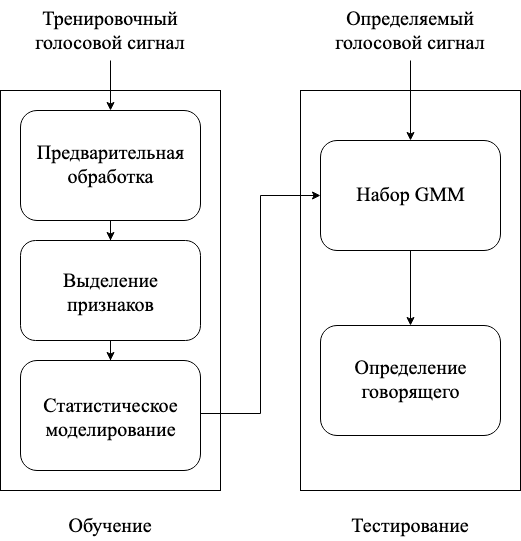
\includegraphics[width=10cm]{./audio_flow.png}
    \caption{Процесс обработки аудиосигнала.}
    \label{fig:audio_flow}
\end{figure}

\newpage
\section{Предварительная обработка аудиосигнала}

Процесс предварительной обработки включает в себя по меньшей мере \cite{jin_noise_mfcc} следующие критически важные шаги:
\begin{enumerate}
    \item \textit{Фрейминг} (\textit{англ.} framing) --- процесс разрезания входного сигнала (записи человеческой речи) на фрагменты.
        Так как речь --- это нестационарный сигнал, её частотное содержание непрерывно изменяется во времени.
        Поэтому для проведения любого анализа предварительно необходимо разбить её на фреймы (части аудиосигнала, ограниченные определёнными временными отрезками), в рамках которых сигнал можно считать стационарным.
        Как правило, для этого достаточно разбить входной поток на фреймы длительностью по $20$--$30$ мс каждый --- можно считать, что форма нашего голосового тракта практически не изменяется за столь малое время.
        Фреймы меньшей длительности уже могут не содержать достаточно информации для получения хорошего приближения частотных компонент, а большей --- уже могут потерять свойство стационарности.
    \item \textit{Экранирование} --- процесс экранирования сигнала на краях фреймов.
        В виду того, что фрейминг звукового сигнала неизбежно приводит к разрывам на краях полученных фреймов, спектральная картина силь искажается.
        Чтобы решить эту проблему, предлагается экранировать каждый фрейм или <<создать окно>> --- уменьшать амплитуду сигнала путём амплитудной модуляции --- на краях фрейма так, чтобы в самых начале и конце фрейма амплитуда была равна нулю, таким образом устраняя разрывы на краях каждого фрейма.
    \item \textit{Добавление пересечения фреймов}.
        Из-за экранирования мы теряем существенную часть частотной информации в начале и в конце каждого фрейма, что так же может привести к некорректной аппроксимации частотной характеристики.
        Чтобы компенсировать потери в количестве данных, вместо того, чтобы делить аудиосигнал на строго непересекающиеся последовательные фреймы, мы позволим им пересекаться так, чтобы теряющийся конец $i$-го фрейма лежал около середины в $(i+1)$-м фрейме.
        Как правило, длительность пересечения принимается равной $10$--$15$ мс.
\end{enumerate}

Рассмотренные количественные параметры можно варьировать и подбирать для получения лучшего приближения.

\section{Выделение признаков}

Следующим обязательным этапом является выделение из входного аудиопотока признаков и формирование его вектора для дальнейшего обучения модели гауссовых смесей.
В качестве признаков как правило \cite{vr_ml, gr_unc_env} выступают \textit{мел-частотные кепстральные коэффициенты} (MFCC --- Mel-Frequency Cepstral Coefficients).
Сперва ответим на вопрос: что эти коэффициенты из себя представляют?

Для дальнейших выкладок нам так или иначе потребуется преобразование Фурье.
Хотя нормировочный множитель нас не будет интересовать, и мы не будем непосредственно проводить вычислений с использованием явного вида преобразования, тем не менее, договоримся о его форме
\begin{equation}
    (\mathcal{F} f)(\omega) \equiv \mathcal{F}(\omega) = \int_{-\infty}^{+\infty} f(t) e^{-2 \pi i \omega t}
\end{equation}
$\forall \omega \in \mathbb{R}$. Тогда обратное преобразование мы получаем
\begin{equation}
    f(t) = \int_{-\infty}^{+\infty} \mathcal{F}(\omega) e^{2 \pi i \omega t}.
\end{equation}

\textit{Кепстр} представляет собой определённый вид гомоморфной обработки сигнала.
Его функция представляет собой обратное преобразование Фурье от логарифма спектра мощности сигнала
\begin{equation}
    C_s(q) = \frac{1}{2 \pi} \int_{-\infty}^{+\infty} \ln |S(\omega)|^2 e^{i \omega q},
\end{equation}
где $S(\omega)$ --- спектр входного сигнала.
Величина $q$, имеющая размерность времени, однако, не несёт здесь привычного смысла и носит название <<кефренс>> (\textit{англ.} quefrency) или <<сачтота>>.

\textit{Мелы} --- это единица измерения частоты, определяемая эмпирической формулой
\begin{equation}\label{eq:ftom}
    m \approx 2595 \log_{10} \left( 1 + \frac{f}{700} \right) \approx 1127 \ln \left( 1 + \frac{f}{700} \right).
\end{equation}
Соответственно, обратное преобразование
\begin{equation}
    f \approx 700 \left( 10^{\frac{m}{2595}} - 1 \right) \approx 700 \left( e^{\frac{m}{1127}} - 1 \right).
\end{equation}

Эта шкала, названная по первым буквам со слова <<мелодия>>, представляет собой психофизическую единицу измерения высоты звука и применяется главным образом в музыкальной акустике.
Её основное свойство --- количественное сохранение психофизического ощущения одинаковой разницы в высоте двух звуков при одновременном сдвиге этих звуков по частотной шкале.
Другими словами, если мы прослушаем две ноты с частотами, скажем, $100$ Гц и $200$ Гц ($\Delta = 100$ Гц), запомним наше ощущение, а затем прослушаем ноты с частотами выше, например, $3000$ Гц и $3100$ Гц ($\Delta = 100$ Гц по-прежнему), нам будет казаться, что последние две ноты отличаются по высоте звука немного, тогда как первые две --- совсем наоборот, и мелы призваны <<уравнять>> наши ощущения и численное значение высоты звука.
Фундаментально этот эффект связан с тем, что привычная нам шкала частот является в самом деле логарифмической, что мы и учитываем в формуле для шкалы мел.

Перейдём теперь к вычислению мел-частотных кепстральных коэффициентов.
Звук является не более чем продольными колебаниями плотности и давления воздуха.
Наш голос представляет собой суперпозицию звука, исходящего прямо из наших лёгких, что является общей чертой всех людей, и звука, промодулированного нашим вокальным трактом, чей спектр, в свою очередь, является уникальным свойством каждого отдельно взятого человека.
Мел-частотные кепстральные коэффициенты примечательны тем, что они как раз и помогают нам разграничить и математически охарактеризовать источник и фильтр нашего голоса.
Для их вычисления нам понадобится выполнить следующую последовательность действий:
\begin{enumerate}
    \item Применить преобразование Фурье к поступившему сигналу, зависящему от времени.
        В частотном пространстве мы теперь имеем следующее замечательное свойство преобразования Фурье:
        \begin{equation}
            \left(\mathcal{F} (s + f) \right) = (\mathcal{F} s) \cdot (\mathcal{F} f),
        \end{equation}
        где $s$ --- функция источника, наших лёгких (source), а $f$ --- функция фильтра, нашего голосового тракта (filter).
        Переведём единицы частоты в мелы, пользуясь (\ref{eq:ftom}).

    \item Логарифмируем полученное выражение, таким образом превращая умножение в суммирование
        \begin{equation}
            \ln \left( (\mathcal{F} s) \cdot (\mathcal{F} f) \right) = \ln (\mathcal{F} s) + \ln (\mathcal{F} f).
        \end{equation}

    \item Наконец, применим дискретное косинус-преобразование Фурье (его использование показало себя более успешным, чем быстрое преобразование Фурье или обратное к нему).
        Изначальный замысел заключается в приведении нашего выражения обратно к временным единицам, однако логарифм не линеен, а, следовательно, новые полученные нами величины уже не имеют смысла времени в привычном понимании --- только по размерности.
        Именно эти величины мы и назвали ранее кефренсами.
\end{enumerate}

\section{Модель гауссовых смесей}

В качестве алгоритма кластеризации мы выберем хорошо зарекомендовавшую себя \cite{hindi_gmm} модель гауссовых смесей, представляющую собой взвешенную сумму гауссовых распределений
\begin{equation}
    p(x | \lambda) = \sum_{i = 1}^K w_i p_i(x | \mu_i, \Sigma_i),
\end{equation}
где веса $w_i$ такие, что $\sum_{i = 1}^K w_i = 1$, и параметры нормального распределения $p_i$ среднее $\mu_i$ и корреляционная матрица $\Sigma_i$ --- искомый набор параметров $\lambda = (w_i, \mu_i, \Sigma_i)_{i = 1}^K$.
\begin{equation}
    p_i(x | \mu_i, \Sigma_i) = \frac{1}{\sqrt{2 \pi |\Sigma_i|}} \exp \left\{ \frac{1}{2} (x - \mu_i)^T \Sigma_i^{-1} (x - \mu_i) \right\}.
\end{equation}

В основе модели лежит предположение, что вероятность пришедшей случайной величины принадлежать одному из кластеров определяется взвешенной суммой гауссовых распределений, каждое из которых описывает один из кластеров.
Сразу же становятся очевидны недостатки такой модели в приложении к голосовой идентификации: во-первых, нам необходимо вручную выбирать количество кластеров (компонентов модели).
Как правило, выбор колеблется от десяти до двадцати компонент в зависимости от типа решаемой задачи.
Во-вторых, использование такой модели ограничивает нас решением лишь замкнутой задачи, когда выбор личности претендента производится из конечного множества заранее записанных людей без возможности определить <<нового>> человека, ещё не прошедшего внесение в базу данных известных нам людей.
Оба эти недостатка, тем не менее, имеют своё разрешение.
От первого можно избавиться, используя специализированные алгоритмы по подбору скрытых параметров в моделях машинного обучения, а от второго --- используя доработанную GMM, называемую GMM-UBM (Gaussian Mixture Model Universal Background Model) \cite{gmm_ubm_smartphone, gmm_ubm_hindi, forensic_gmm_ubm_mfcc}, которая учитывает общие черты большого количества людей и определяет, когда претендент принадлежит общей <<фоновой>> модели, а когда --- является конкретной личностью из заранее записанных.
В настоящей работе мы не будем касаться реализации этих методов и ограничимся лишь замечанием об их существовании.

\section{Тренировка модели}

Модель обычно инициализирована $K$ кластерами алгоритма $k$-средних с одинаковыми весами $w_i \equiv \frac{1}{K}$.
$K$ гауссовых распределений размещены по этим кластерам.
Далее параметры модели последовательно обновляются до достижения сходимости.

Наиболее популярный алгоритм нахождения параметров носит название алгоритма максимизаци ожидания (EM --- Expectation Maximization) \cite{em_new}.
В общем виде алгоритм представляет из себя итеративную процедуру максимизации матожидания логарифма правдоподобия.
Пусть нам даны значения наблюдаемых переменных $X$ и набор латентных переменных $T$, вместе образующих полный набор данных.
Здесь $T$ и будет являться неким знанием о задаче.
Скажем, взвешенной смесью гауссовых распределений.
Тогда положим $p$ плотностью вероятности полного набора данных с параметрами $\Theta$: $p(X)$ --- функция правдоподобия модели, зависящая от параметра $\Theta$.
Используя расширенную формулу Байеса и формулу полной вероятности, имеем
\begin{equation}
    p(T | X, \Theta) = \frac{p(X | T, \Theta) \cdot p(T | \Theta)}{\int p(X | T', \Theta) \cdot p(T' | \Theta) d T'},
\end{equation}
в виду чего нам необходимо знать только лишь распределение наблюдаемой компоненты при фиксированной скрытой $p(X | T, \Theta)$ и вероятности скрытых данных $p(T, \Theta)$.

EM-алгоритм итеративно улучшает начальную оценку $Theta_0$, делая переход от $\Theta_i$ к $\Theta_{i + 1}$ по формуле
\begin{equation}
    \Theta_{i + 1} = \arg \max_\Theta Q(\Theta),
\end{equation}
где $Q(\Theta) = E_T \left[ \log p(X, T | \Theta) \mid X \right]$ --- матожидание логарифма правдоподобия (условное матожидание $\log p(X, T | \Theta)$ при условии $X$), о котором говорилось ранее.
Таким образом, по исходным данным $X$ мы находим апостериорную оценку вероятностей для различных значений скрытых переменных $T$.

\section{Замечания}

Часто для уточнения модели помимо самих MFCC используют и аппроксимации их производных, что существенно увеличивает точность модели.

Одна модель тренируется для одного человека.
Таким образом, мы набираем мел-частотные кепстральные коэффициенты для всех фреймов семпла голоса одного данного человека, собираем их в несколько векторов, где размер вектора (количество признаков) равен числу MFCC.
Затем на полученной матрице с помощью EM-алгоритма мы тренируем модель гауссовых смесей и переходим.
Процесс повторяется для всех выбранных людей.

Тот же самый метод можно применить для определения, скажем, пола человека.
В этом случае нам потребуется всего две модели гауссовых смесей, одна --- для мужского пола, а другая --- для женского.

Построив необходимое число моделей, переходим к следующему этапу.

\newpage
\section{Тестирование модели}

После получения нами натренированной модели для выбранных людей, выясним, кем является автор пришедшего тестового высказывания.
Для этого с помощью построенных моделей необходимо получить оценки вероятностей появления данного высказывания с его характеристиками в каждой из моделей.
Тогда мы можем выяснить (с некоторой вероятностью) личность автора высказывания как автора натренированной модели с наибольшей итоговой вероятностью.

Более формально, для каждого фрейма тестового высказывания мы считаем вероятность того, что этот фрейм принадлежит данной модели
\begin{equation}
    p(x_j | \lambda_k) = \sum_{i = 1}^K p_i(x | \mu_i^{(k)}, \Sigma_i^{(k)}),
\end{equation}
где индекс $k$ указывает проверяемую модель (личность), а индекс $j$ нумерует фреймы тестового высказывания.
Получив $p(x_j | \lambda_k)$ для всех $j$, мы можем теперь для каждой модели сложить логарифмы полученных вероятностей для каждого фрейма и получить распределение, максимум которого и укажет нам наиболее вероятную личность
\begin{equation}
    S_k = \sum_j \log p(x_j | \lambda_k) \text{, } k' = \arg \max_k S_k,
\end{equation}
где $k'$ обозначен результат тестирования.

\section{Программная реализация}

Демонстрационные прототипы программ реализованы на языке программирования Python, так как он является наиболее подходящим языком для решения задач с приложениями алгоритмов машинного обучения.
Исходный код обеих программ можно видеть в приложениях.
Кратко опишем в этом разделе архитектуру обоих программных продуктов.

\newpage
\section{Распознавание пола}

Программа по распознаванию пола состоит из двух основных модулей:
\begin{itemize}
    \item Модуль создания и тренировки модели гауссовых смесей.
    \item Модуль обработки голоса и выделения мел-частотных кепстральных коэффициентов.
\end{itemize}

Модули объединены общей программой, получающей на вход набор высказываний мужского и женского голосов, и на высоком уровне уровне реализующей получение двух натренированных моделей и определение их точности по тестовым высказываниям из другого датасета.
Для упрощения кода, пользуясь небольшими размерами датасета, сохранение модели в отдельный файл опущено.
В реалистичных сценариях, конечно, модель необходимо сохранять и хранить отдельно от программы, так как её перетренировка может занимать много времени.

\section{Распознавание голоса}

Рассмотрим теперь программу по распознаванию голоса.
Архитектурно она не сильно отличается от программы для распознавания пола говорящего, однако изменения затронули процесс сбора признаков.
Теперь помимо мел-частотных кепстральных коэффициентов мы вычисляем их разности, аппроксимируя таким образом с точностью до некоторой константы производные этих коэффициентов.
В модели для распознавания пола это не играло такой важной роли, потому что наша задача в известном смысле сводилась к бинарной классификации.
Здесь же мы вынуждены выбирать в общем случае из сколь угодно большого набора натренированных моделей, что делает учёт производных мел-частотных кепстральных коэффициентов необходимым.

\newpage
\conclusion

В ходе работы был рассмотрен и реализован алгоритм голосовой идентификации на основе модели гауссовых смесей с использованием мел-частотных кепстральных коэффициентов и их производных в качестве вектора признаков.
Для определения параметров модели был использован алгоритм максимизации ожидания.

В рамках выбранной модели были получены количественные оценки вероятности распознавания пола человека:
\begin{itemize}
    \item Женская модель: 90\%.
        Наилучший результат: 96\%.
    \item Мужская модель: 60\%.
        Наилучший результат: 67\%
    \item Порядок общей точности системы: 80\%.
\end{itemize}

В обучающую выборку вошли по 5 минут мужских и женских разговоров.
В тестовой выборке находились относительно короткие (10--15 секунд) высказывания разных полов с низким уровнем шума.
На результат оказали влияние как скрытые параметры модели, так и выборка обучающих и тестовых высказываний.

В рамках той же модели была получена оценка вероятности распознавания личности из группы размером 34 человека.
Для каждого говорящего имелось по 10 различных высказываний, из которых 5 являлись обучающими, и 5 --- тестовыми.
Говорящие за пределами данного датасета рассмотрены не были.
Полученная оценка вероятности определения человека по голосу в данной модели составила 50\%.

\newpage
\references

\bibliographystyle{gost780u}
\bibliography{bibliography}

% \newpage
% \addcontentsline{toc}{section}{ПРИЛОЖЕНИЕ А Реализация прототипа программы по распознаванию пола}
% \section*{ПРИЛОЖЕНИЕ А}

% \begin{center}
%     \large
%     \textbf{Реализация прототипа программы по распознаванию пола}
% \end{center}

%\lstinputlisting[language=Python, caption={\centering \textit{ml.py} --- создание и тренировка модели.}]{./gender-recognition/ml.py}


%\newpage
%\lstinputlisting[language=Python, caption={\centering \textit{voice\_processing.py} --- обработка голоса. Выделение и нормализация признаков из звукового потока.}]{./gender-recognition/voice-processing.py}

%\newpage
%\lstinputlisting[language=Python, caption={\centering \textit{main.py} --- основная программа, производящая вычисления точностей.}]{./gender-recognition/main.py}

%\newpage
%\addcontentsline{toc}{section}{ПРИЛОЖЕНИЕ Б Реализация прототипа программы по распознаванию голоса}
%\section*{ПРИЛОЖЕНИЕ Б}

%\begin{center}
%    \large
%    \textbf{Реализация прототипа программы по распознаванию голоса}
%\end{center}

% \lstinputlisting[language=Python, caption={\centering \textit{ml.py} --- создание и тренировка модели.}]{./voice-recognition/ml.py}

% \newpage
% \lstinputlisting[language=Python, caption={\centering \textit{features.py} --- обработка голоса. Выделение и нормализация признаков из звукового потока. По сравнению с определением пола мы добавили новый признак --- разность мел-частотных кепстральных коэффициентов. Таким образом, величина вектора признаков фрейма возросла.}]{./voice-recognition/features.py}

% \newpage
% \lstinputlisting[language=Python, caption={\centering \textit{main.py} --- основная программа, производящая вычисления точности.}]{./voice-recognition/main.py}

\end{document}
